% ============================================================
%  Portfolio Optimization with Black-Litterman
%  Technical Report
% ============================================================
\documentclass[11pt, a4paper]{article}

% ── Page geometry ───────────────────────────────────────────
\usepackage[top=2.5cm, bottom=2.5cm, left=2.8cm, right=2.8cm]{geometry}

% ── Fonts & encoding ────────────────────────────────────────
\usepackage[T1]{fontenc}
\usepackage[utf8]{inputenc}
\usepackage{lmodern}
\usepackage{microtype}

% ── Math ────────────────────────────────────────────────────
\usepackage{amsmath, amssymb, bm}

% ── Tables ──────────────────────────────────────────────────
\usepackage{booktabs}
\usepackage{array}
\usepackage{colortbl}
\newcolumntype{L}[1]{>{\raggedright\arraybackslash}p{#1}}
\newcolumntype{C}[1]{>{\centering\arraybackslash}p{#1}}
\newcolumntype{R}[1]{>{\raggedleft\arraybackslash}p{#1}}

% ── Colours ─────────────────────────────────────────────────
\usepackage{xcolor}
\definecolor{blnavy}{RGB}{26,  73, 101}
\definecolor{blamber}{RGB}{202,103,  2}
\definecolor{blteal}{RGB}{ 42,157, 143}
\definecolor{blgrey}{RGB}{245,245,248}

% ── Graphics / TikZ ─────────────────────────────────────────
\usepackage{graphicx}
\usepackage{tikz}
\usetikzlibrary{arrows.meta, positioning, shapes.geometric}

% ── Code ─────────────────────────────────────────────────────
\usepackage{verbatim}
\usepackage{fancyvrb}
\fvset{fontsize=\small, frame=single, framesep=4pt,
       rulecolor=\color{blnavy!30}}

% ── Section styling ─────────────────────────────────────────
\usepackage{titlesec}
\titleformat{\section}
  {\large\bfseries\color{blnavy}}{\thesection}{0.8em}{}[\vspace{-4pt}\textcolor{blnavy}{\rule{\linewidth}{0.5pt}}]
\titleformat{\subsection}
  {\normalsize\bfseries\color{blnavy!80}}{\thesubsection}{0.8em}{}

% ── Callout box ─────────────────────────────────────────────
\usepackage{tcolorbox}
\tcbuselibrary{skins}
\newtcolorbox{researchbox}{
  colback=blnavy!6, colframe=blnavy,
  boxrule=0.6pt, arc=3pt,
  left=8pt, right=8pt, top=6pt, bottom=6pt,
  fonttitle=\bfseries\small\color{white},
  title=Core Research Question,
  attach boxed title to top left={yshift=-2pt, xshift=8pt},
  boxed title style={colback=blnavy, arc=2pt, boxrule=0pt}
}
\newtcolorbox{limitbox}{
  colback=blamber!8, colframe=blamber,
  boxrule=0.6pt, arc=3pt,
  left=8pt, right=8pt, top=6pt, bottom=6pt,
  fonttitle=\bfseries\small\color{white},
  title=Known Model Limitation,
  attach boxed title to top left={yshift=-2pt, xshift=8pt},
  boxed title style={colback=blamber, arc=2pt, boxrule=0pt}
}
\newtcolorbox{notebox}{
  colback=blteal!6, colframe=blteal,
  boxrule=0.6pt, arc=3pt,
  left=8pt, right=8pt, top=6pt, bottom=6pt,
}

% ── Headers & footers ────────────────────────────────────────
\usepackage{fancyhdr}
\pagestyle{fancy}
\fancyhf{}
\renewcommand{\headrulewidth}{0.4pt}
\fancyhead[L]{\small\textcolor{blnavy}{Portfolio Optimization with Black-Litterman}}
\fancyhead[R]{\small\textcolor{blnavy!60}{\thepage}}
\renewcommand{\headrule}{\color{blnavy!30}\hrule width\headwidth height\headrulewidth}

% ── Hyperlinks ───────────────────────────────────────────────
\usepackage[
  colorlinks=true,
  linkcolor=blnavy,
  urlcolor=blteal,
  citecolor=blnavy,
  pdfauthor={},
  pdftitle={Portfolio Optimization with Black-Litterman},
]{hyperref}

% ── Spacing helpers ─────────────────────────────────────────
\setlength{\parskip}{5pt}
\setlength{\parindent}{0pt}

% ── Helpers ─────────────────────────────────────────────────
\newcommand{\BL}{\mathrm{BL}}
\newcommand{\code}[1]{\texttt{#1}}

% ============================================================
\begin{document}
% ============================================================

% ── Title block ─────────────────────────────────────────────
\begin{center}
  {\LARGE\bfseries\color{blnavy}
    Portfolio Optimization with Black-Litterman}\\[8pt]
  {\large A Case Study in Public Portfolio Disclosures}\\[10pt]
  \textcolor{blnavy!50}{\rule{0.6\linewidth}{0.5pt}}\\[6pt]
  \small\textcolor{blnavy!70}{
    Walk-forward backtest $\cdot$ Real SEC \& congressional filing data
    $\cdot$ Buffett $\cdot$ Pelosi $\cdot$ Trump}
\end{center}

\vspace{8pt}

% ── Abstract ─────────────────────────────────────────────────
\begin{tcolorbox}[colback=blgrey, colframe=blnavy!20, arc=3pt,
                  boxrule=0.4pt, left=10pt, right=10pt,
                  top=8pt, bottom=8pt]
  \small\textbf{Abstract.}\;
  This report describes a Python codebase that applies a Black-Litterman
  portfolio overlay to publicly disclosed equity holdings and evaluates it
  in a rolling walk-forward backtest. Three case studies are constructed from
  real regulatory filings --- Berkshire Hathaway SEC~13F (Warren Buffett),
  U.S.\ House Financial Disclosure (Nancy Pelosi), and OGE~278e
  (Donald Trump) --- and three strategies are compared: a static
  disclosed-weight portfolio, a sample mean-variance optimiser, and a
  Black-Litterman posterior fed into a long-only quadratic programme.
  The framework is fully YAML-configurable, ships with 63 unit and
  integration tests, and produces four analysis notebooks covering data
  quality, strategy comparison, hyperparameter sensitivity, and benchmark
  attribution.
\end{tcolorbox}

\tableofcontents
\vspace{6pt}
\textcolor{blnavy!20}{\rule{\linewidth}{0.4pt}}

% ============================================================
\section{Motivation and Research Question}
% ============================================================

Three distinct regulatory filing regimes require institutional investors and
public officials to disclose their equity holdings: the SEC~13F form
(institutional investment managers with $\geq\$100$M AUM), the U.S.\ House
Financial Disclosure report (members of Congress), and the U.S.\ Office of
Government Ethics~278e annual disclosure (executive-branch officials).
Although these filings differ in granularity and timing, each provides a
public record of approximate portfolio weights that can serve as an
\emph{investor view} within a quantitative portfolio construction framework.

\medskip
\begin{center}
\begin{tabular}{@{}lll@{}}
  \toprule
  \textbf{Person} & \textbf{Filing type} & \textbf{Source} \\
  \midrule
  Warren Buffett  & SEC 13F               & Berkshire Hathaway, as of 2025-12-31 \\
  Nancy Pelosi    & House FD report       & Report 10066169; midpoints of ranges \\
  Donald Trump    & OGE 278e              & Annual disclosure; midpoints / lower bounds \\
  \bottomrule
\end{tabular}
\end{center}
\medskip

Range-based values (which appear in both House~FD and OGE~278e filings) are
converted to midpoints where both bounds are available, and to the reported
lower bound otherwise.

\begin{researchbox}
  Can a Black-Litterman overlay improve portfolio quality relative to:\\[4pt]
  \quad (1) the \textbf{disclosed} portfolio itself (passive replication)?\\[2pt]
  \quad (2) a \textbf{mean-variance} (sample-estimated Markowitz) baseline?\\[6pt]
  \textit{Improvement} is assessed on annualised Sharpe ratio, Sortino ratio,
  maximum drawdown, HHI concentration, and average turnover.
\end{researchbox}

% ============================================================
\section{Data Pipeline}
% ============================================================

The pipeline ingests two CSV files --- holdings disclosures and adjusted
daily prices --- and produces a \code{CaseStudyResult} dataclass containing
the three \code{BacktestResult} objects, one per strategy. Figure~\ref{fig:pipeline}
summarises the flow.

\begin{figure}[h]
\centering
\resizebox{\linewidth}{!}{%
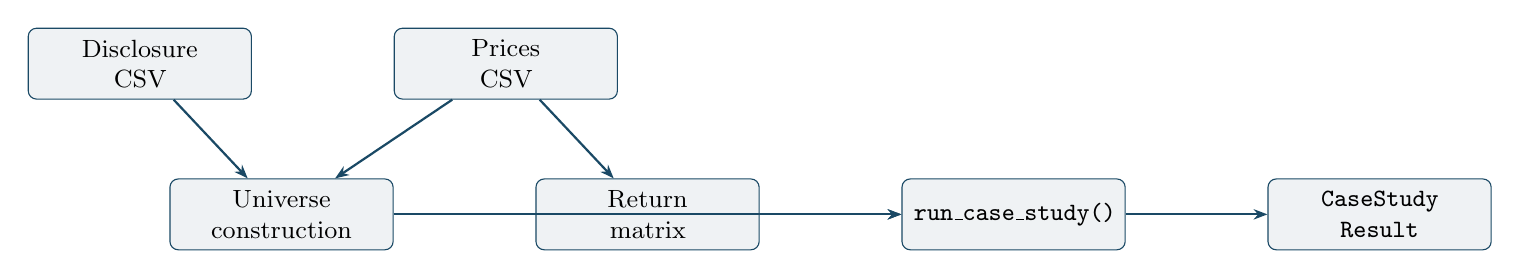
\begin{tikzpicture}[
    node distance=1.0cm and 1.8cm,
    box/.style={draw=blnavy, rounded corners=3pt, fill=blnavy!7,
                text width=2.6cm, align=center,
                minimum height=0.9cm, font=\small},
    arr/.style={-{Stealth[length=5pt]}, blnavy, thick}
  ]
  \node[box] (disc)   {Disclosure\\CSV};
  \node[box, right=of disc] (prices) {Prices\\CSV};
  \node[box, below=of disc, xshift=1.8cm] (univ) {Universe\\construction};
  \node[box, right=of univ]  (ret)  {Return\\matrix};
  \node[box, right=of ret]   (pipe) {\code{run\_case\_study()}};
  \node[box, right=of pipe]  (res)  {\code{CaseStudy\\Result}};

  \draw[arr] (disc)   -- (univ);
  \draw[arr] (prices) -- (univ);
  \draw[arr] (prices) -- (ret);
  \draw[arr] (univ)   -- (pipe);
  \draw[arr] (ret)    -- (pipe);
  \draw[arr] (pipe)   -- (res);
\end{tikzpicture}}%
\caption{End-to-end data pipeline. Both CSV files are validated on load before
any modelling occurs.}
\label{fig:pipeline}
\end{figure}

\subsection{Disclosures (\code{data/disclosures.py})}

\code{load\_disclosures\_csv()} schema-validates the input on load, dropping
any rows with missing or non-positive weights and emitting a warning for each
dropped row.\\
\code{latest\_portfolio\_for\_aliases()} selects the most recent
filing date for a given set of ticker aliases, ensuring that the disclosed
weights reflect the latest available snapshot without introducing any look-ahead
bias relative to the price history.

\subsection{Prices (\code{data/prices.py})}

The price dataset covers 46 tickers from 2018-01-02 to 2025-12-30 using
split- and dividend-adjusted daily closing prices sourced from Yahoo Finance.
\code{load\_prices\_csv()} detects and warns on duplicate \code{(date, ticker)}
pairs. \code{to\_return\_matrix()} pivots the long-format price table into
a wide daily log-return matrix aligned to the backtest calendar.

% ============================================================
\section{Three Strategies}
% ============================================================

All three strategies share the same asset universe, lookback window, rebalance
schedule, and long-only constraint, ensuring that any observed performance
differences are attributable to the portfolio construction method alone.

\medskip
\begin{center}
\begin{tabular}{@{}L{2.8cm} L{10cm}@{}}
  \toprule
  \textbf{Strategy} & \textbf{Description} \\
  \midrule
  \textbf{Disclosed} &
    Static buy-and-hold of the filed portfolio weights. No rebalancing occurs;
    turnover is zero. This represents an upper bound on what a fully passive
    follower of the public disclosure can achieve. \\[6pt]
  \textbf{Mean-Variance} &
    Long-only Markowitz optimisation using the sample mean and covariance
    estimated over the lookback window. This is the classical quantitative
    benchmark, known to be sensitive to estimation error in the mean. \\[6pt]
  \textbf{Black-Litterman} &
    Equilibrium prior blended with disclosure-implied views to form a
    posterior expected return vector and covariance matrix, which are then
    passed to the same long-only quadratic programme. This is the primary
    strategy under investigation. \\
  \bottomrule
\end{tabular}
\end{center}

% ============================================================
\section{The Black-Litterman Model}
% ============================================================

\subsection{Equilibrium Prior}

The Black-Litterman framework begins by computing the \emph{implied equilibrium
excess return vector} by reverse-engineering the market-clearing condition.
Given market-cap proxy weights $\bm{w}_{\text{mkt}}$, risk-aversion scalar
$\lambda$, and asset covariance matrix $\bm{\Sigma}$:
\begin{equation}
  \bm{\pi} = \lambda\,\bm{\Sigma}\,\bm{w}_{\text{mkt}}
  \label{eq:pi}
\end{equation}
with $\lambda = 2.5$ (default). These equilibrium returns serve as the
prior mean for the distribution of expected returns.

\subsection{Views from Disclosures}

The disclosed portfolio weights define a single \emph{absolute view}: the
investor's filed holdings implicitly express a belief about relative expected
returns. The view-picking matrix $P$ ($k \times n$) extracts the relevant
linear combination of assets, and the view return vector $\bm{q}$ encodes the
expected return of that combination. View uncertainty is modelled as
proportional to the prior covariance:
\begin{equation}
  \bm{\Omega} = \frac{1 - c}{c}\,P\bm{\Sigma}P^{\top}
  \label{eq:omega}
\end{equation}
where $c \in (0, 1)$ is the \textbf{view\_confidence} parameter (default:
$0.65$). As $c \to 1$ the posterior collapses to the disclosed view; as
$c \to 0$ it collapses to the equilibrium prior.

\subsection{Posterior Update}

Following He and Litterman (1999), the posterior is derived analytically.
Define the posterior precision matrix:
\begin{equation}
  M = (\tau\bm{\Sigma})^{-1} + P^{\top}\bm{\Omega}^{-1}P
  \label{eq:M}
\end{equation}
where $\tau = 0.05$ (default) controls the uncertainty in the prior.
The posterior mean and covariance are:
\begin{align}
  \bm{\mu}_{\BL} &= M^{-1}\Bigl[
    (\tau\bm{\Sigma})^{-1}\bm{\pi} + P^{\top}\bm{\Omega}^{-1}\bm{q}
  \Bigr]
  \label{eq:muBL} \\[6pt]
  \bm{\Sigma}_{\BL} &= \bm{\Sigma} + M^{-1}
  \label{eq:SigmaBL}
\end{align}

The pair $(\bm{\mu}_{\BL},\,\bm{\Sigma}_{\BL})$ is then passed to a
long-only quadratic programme with the full-investment constraint
$\mathbf{1}^{\top}\bm{w} = 1$, $\bm{w} \geq 0$. If the solver returns
all non-positive weights the strategy falls back to equal-weight allocation
and logs a warning.

\medskip
\begin{center}
\begin{tabular}{@{}cl@{}}
  \toprule
  \textbf{Symbol} & \textbf{Meaning} \\
  \midrule
  $\lambda$      & Risk-aversion scalar (default: $2.5$) \\
  $\tau$         & Prior uncertainty scalar (default: $0.05$) \\
  $c$            & View confidence (default: $0.65$; swept in Notebook 03) \\
  $P$            & $k \times n$ view-picking matrix \\
  $\bm{q}$       & $k$-vector of view returns \\
  $\bm{\Omega}$  & $k \times k$ view uncertainty matrix \\
  \bottomrule
\end{tabular}
\end{center}

% ============================================================
\section{Walk-Forward Backtest Engine}
% ============================================================

\subsection{Design and Lookahead-Bias Prevention}

\code{rolling\_backtest()} in \code{backtest/engine.py} implements a strict
no-lookahead-bias design: at each month-end rebalance date $t$, portfolio
weights are computed using only the 6-month trailing window of returns ending
at $t$, and those weights are applied to returns \emph{starting from the
period after} $t$. The \code{weight\_history} output is indexed by decision
date, making it straightforward to audit the lag.

\subsection{Configuration}

All hyperparameters are declared in \code{configs/case\_studies.yaml} and
loaded into a frozen \code{BacktestConfig} dataclass at runtime. No magic
numbers appear in the source code.

\medskip
\begin{center}
\begin{tabular}{@{}ll@{}}
  \toprule
  \textbf{Parameter} & \textbf{Value} \\
  \midrule
  \code{lookback\_periods}    & 6 months \\
  \code{rebalance\_frequency} & Month-end (\code{ME}) \\
  \code{risk\_aversion}       & $\lambda = 2.5$ \\
  \code{tau}                  & $\tau = 0.05$ \\
  \code{view\_confidence}     & $c = 0.65$ \\
  \bottomrule
\end{tabular}
\end{center}

\subsection{Output}

\code{rolling\_backtest()} returns a \code{BacktestResult} dataclass with
three fields: \code{.returns} (daily return series), \code{.nav}
(cumulative NAV indexed from 1.0), and \code{.weight\_history}
(DataFrame of rebalance-date weights).

% ============================================================
\section{Performance Metrics}
% ============================================================

All metrics are computed by \code{backtest/metrics.py}. The helper
\code{infer\_periods\_per\_year()} automatically detects daily, monthly,
or quarterly frequency from the return index and emits a \code{UserWarning}
when fewer than three observations are available.

\medskip
\begin{center}
\begin{tabular}{@{}L{3.6cm} L{9.5cm}@{}}
  \toprule
  \textbf{Metric} & \textbf{Notes} \\
  \midrule
  Annual return    & Geometric compounding from NAV series. \\
  Annual volatility & Annualised standard deviation of daily returns. \\
  Sharpe ratio     & Excess return over annualised volatility; risk-free
                     rate defaults to zero. \\
  Sortino ratio    & Excess return over downside deviation; returns
                     \code{nan} (not $+\infty$) when no negative daily
                     return exists in the window, avoiding misleading
                     statistics on strongly trending periods. \\
  Max drawdown     & Maximum peak-to-trough decline in cumulative NAV. \\
  HHI concentration & $\sum_i w_i^2$; ranges from $1/n$ (equal-weight)
                     to $1.0$ (fully concentrated). \\
  Average turnover  & Mean $L_1$ weight change per rebalance:
                     $\frac{1}{T}\sum_t \|\bm{w}_t - \bm{w}_{t-1}\|_1$. \\
  \bottomrule
\end{tabular}
\end{center}

\code{summarize\_strategy()} aggregates all seven metrics into a dict, which
the notebooks collect into a combined summary DataFrame for side-by-side
comparison across strategies and persons.

% ============================================================
\section{Analysis Notebooks}
% ============================================================

The repository ships four Jupyter notebooks. All notebooks iterate over the
\textbf{Buffett}, \textbf{Pelosi}, and \textbf{Trump} case studies from a
shared \code{results} dict --- no person keys are hardcoded.

\subsection{Notebook 01 --- Data Quality \& Universe Overview}

Performs schema checks on the raw holdings and price CSVs, reports holdings
coverage (fraction of disclosed tickers with matching price history), and
renders portfolio composition pie charts for each person. The output provides
a sanity check that the data pipeline has ingested the filings correctly before
any modelling is run.

\subsection{Notebook 02 --- Strategy Comparison Case Study}

The main results notebook. For each person it plots:
\begin{itemize}
  \item Equity curves (cumulative NAV) for all three strategies on a shared axis.
  \item Drawdown time series highlighting the 2020 COVID drawdown and 2022
        rate-shock episodes.
  \item Black-Litterman weight evolution over rebalance dates, showing how the
        posterior allocation shifts as the disclosure-implied view interacts with
        the changing equilibrium prior.
  \item A combined summary table with all seven metrics for all three strategies.
\end{itemize}

\subsection{Notebook 03 --- Black-Litterman Sensitivity Analysis}

Sweeps the view confidence parameter $c \in \{0.20, 0.25, \ldots, 0.95\}$
(16 values) across all three persons, running 48 independent backtests in
total. The results are displayed in a $2 \times 3$ subplot grid showing how
annualised return, volatility, Sharpe ratio, HHI, and average turnover respond
to $c$.

Key findings from the sweep:
\begin{itemize}
  \item The Sharpe ratio is \emph{non-monotonic} in $c$ on real data --- the
        value of $c$ that maximises Sharpe differs across persons and cannot
        be determined a priori.
  \item Higher confidence causes turnover to increase when the disclosed view
        diverges substantially from the equilibrium prior.
  \item HHI spikes near extreme values of $c$, indicating that very high or
        very low confidence produces concentrated allocations.
\end{itemize}

The best-by-Sharpe row is printed for each person, providing a principled
starting range for \code{view\_confidence} before any out-of-sample reporting.

\subsection{Notebook 04 --- Benchmark Attribution \& Alpha Decomposition}

Fits an OLS factor model to each strategy's return series:
\begin{equation}
  r_{\text{strat},t} = \alpha
    + \beta_1 r_{\text{SPY},t}
    + \beta_2 r_{\text{Tech},t}
    + \beta_3 r_{\text{Energy},t}
    + \beta_4 r_{\text{Fin},t}
    + \beta_5 r_{\text{CD},t}
    + \varepsilon_t
  \label{eq:ols}
\end{equation}
where benchmarks are sourced preferentially from ETF tickers (SPY, XLK, XLE,
XLF, XLY) with an automatic fallback to ticker-proxy averages
(e.g.\ AAPL + MSFT + NVDA for Tech) if the ETF is absent from the price
file. A provenance table is printed per person.

For each person the notebook produces:
\begin{itemize}
  \item A $\hat{\beta}$ bar chart (positive loadings in teal, negative in red).
  \item An arithmetic return contribution decomposition:
        $\bar{r}_{\text{ann}} \approx \hat{\alpha}\cdot f + \sum_k \hat{\beta}_k \bar{r}_{k,\text{ann}} + \text{residual}$,
        where $f$ is periods per year.
  \item A return correlation heatmap between the strategy and each factor.
  \item Rolling 12-month $\hat{\alpha}$ and $\hat{\beta}$ versus SPY, revealing
        regime shifts hidden in the full-sample statistics --- most visibly
        during the 2020 COVID drawdown and the 2022 rate shock.
\end{itemize}

% ============================================================
\section{Codebase Architecture}
% ============================================================

\subsection{Package Layout}

The \code{portfolio\_bl} package lives entirely under \code{src/} and is
organised into three sub-packages.

\medskip
\begin{center}
\begin{tabular}{@{}L{5.8cm} L{7.3cm}@{}}
  \toprule
  \textbf{Module} & \textbf{Responsibility} \\
  \midrule
  \code{config.py}                    & YAML loading; \code{BacktestConfig} and
                                        \code{CaseStudyConfig} frozen dataclasses. \\
  \code{pipeline.py}                  & \code{run\_case\_study()} orchestrator;
                                        returns \code{CaseStudyResult}. \\
  \code{data/disclosures.py}          & Load, validate, and filter holdings CSV. \\
  \code{data/prices.py}               & Load prices CSV; pivot to return matrix. \\
  \code{models/black\_litterman.py}   & \code{implied\_equilibrium\_returns()};
                                        \code{black\_litterman\_posterior()}. \\
  \code{models/mean\_variance.py}     & \code{long\_only\_markowitz()} with
                                        equal-weight fallback. \\
  \code{backtest/engine.py}           & \code{rolling\_backtest()} walk-forward loop. \\
  \code{backtest/metrics.py}          & All seven performance metrics;
                                        \code{summarize\_strategy()}. \\
  \bottomrule
\end{tabular}
\end{center}

\subsection{Quality and Observability}

\begin{itemize}
  \item \textbf{63 tests} (unit and integration) runnable with
        \code{pytest --tb=short}. Tests cover the BL posterior algebra,
        backtest engine edge cases (empty windows, all-positive returns),
        and metric correctness.
  \item \code{logging.getLogger(\_\_name\_\_)} is configured in every module.
        The \code{--verbose} flag elevates the log level to \code{DEBUG},
        printing per-rebalance diagnostics without modifying any source file.
  \item \code{FileNotFoundError} and \code{ValueError} are raised with
        descriptive messages on bad or missing inputs; no silent failures.
  \item \code{\_\_all\_\_} is defined in every \code{\_\_init\_\_.py},
        making the public API explicit.
  \item All BL hyperparameters are exposed via YAML; no magic numbers
        appear in the source code.
\end{itemize}

\subsection{CLI Quick-Start}

\begin{Verbatim}
PYTHONPATH=src python scripts/run_case_study.py \
  --config configs/case_studies.yaml \
  --person buffett \
  --verbose
\end{Verbatim}

Swapping \code{--person buffett} for \code{pelosi} or \code{trump} runs
the identical pipeline on a different case study. All three persons can also
be run programmatically by calling \code{run\_case\_study()} in a loop
with different \code{CaseStudyConfig} objects.

% ============================================================
\section{Known Limitation and Extensions}
% ============================================================

\begin{limitbox}
  The BL posterior assumes multivariate Gaussianity in both returns and
  views. Equity return distributions exhibit significant excess kurtosis
  and left-tail asymmetry, particularly during stress periods directly
  visible in this backtest --- the \textbf{2020 COVID drawdown} and the
  \textbf{2022 rate shock}. A production-grade system would replace the
  Gaussian prior with Meucci's Entropy Pooling / Copula Opinion Pooling
  framework, which separates the marginal distributions from the dependence
  structure and allows views to be expressed on arbitrary statistics
  including implied volatility.
\end{limitbox}

\medskip
The practical consequences within this backtest are:
\begin{itemize}
  \item The posterior covariance $\bm{\Sigma}_{\BL}$ underestimates tail risk
        during crisis periods, causing the optimiser to over-allocate to assets
        that appear low-volatility under normality but exhibit fat tails under
        stress.
  \item The Sortino ratio and maximum drawdown are therefore the most
        informative diagnostics in this framework, as they directly capture
        downside behaviour without assuming symmetry.
\end{itemize}

The Entropy Pooling approach is the natural upgrade path: it preserves the
Bayesian blending intuition of Black-Litterman while removing the Gaussian
assumption entirely.

% ============================================================
\section{Summary}
% ============================================================

\begin{notebox}
\textbf{What the framework provides}
\begin{itemize}
  \item End-to-end walk-forward backtest on real, publicly-filed portfolio data
        --- not synthetic or simulated holdings.
  \item Fair three-way strategy comparison: Disclosed, Mean-Variance,
        and Black-Litterman on an identical universe and schedule.
  \item Full sensitivity sweep over the key BL hyperparameter ($c$),
        producing 48 backtests across three persons.
  \item OLS factor attribution with rolling 12-month diagnostics.
  \item YAML-configurable --- swap in any universe or parameter set without
        modifying source code.
  \item 63 tests enforcing correctness at every layer of the stack.
\end{itemize}

\textbf{Key design decisions}
\begin{itemize}
  \item No-lookahead-bias by construction in the engine.
  \item Graceful degradation to equal-weight with a logged warning rather
        than a hard crash.
  \item \code{nan} (not $+\infty$) Sortino on all-positive return periods.
  \item Real adjusted prices (2018--2025, 46 tickers) via Yahoo Finance.
\end{itemize}
\end{notebox}

\vspace{12pt}
\begin{center}
  \textcolor{blnavy!40}{\rule{0.7\linewidth}{0.4pt}}\\[4pt]
  \small\textcolor{blnavy!60}{%
    \texttt{github.com/mengrenman/portfolio-optimization-black-litterman}}
\end{center}

% ============================================================
\end{document}
% ============================================================
